\documentclass[11 pt]{article}

\usepackage[margin=1in]{geometry}

\usepackage{parskip}

\usepackage{amsmath}
\usepackage{amssymb}

\usepackage{graphicx}

\usepackage{array}
\usepackage{booktabs}

\usepackage{microtype}

\usepackage{siunitx}
\usepackage{xspace}

\usepackage{setspace}
% \doublespacing

% \usepackage[compact]{titlesec}

\usepackage[]{appendix}




% \usepackage{newtxtext}
% \usepackage{newtxmath}

% Code packages 
	\usepackage[dvipsnames]{xcolor}

	\usepackage{listings}
	\usepackage{color}

	\definecolor{dkgreen}{rgb}{0,0.3,0}
	\definecolor{gray}{rgb}{0.5,0.5,0.5}
	\definecolor{mauve}{rgb}{0.58,0,0.82}	

	\usepackage{inconsolata}

	\lstset{frame=tb,
	  language=Python,
	  aboveskip=3mm,
	  belowskip=3mm,
	  showstringspaces=false,
	  columns=flexible,
	  basicstyle={\small\ttfamily},
	  numbers=none,
	  numberstyle=\tiny\color{gray},
	  keywordstyle=\color{blue},
	  commentstyle=\color{dkgreen},
	  stringstyle=\color{mauve},
	  breaklines=true,
	  breakatwhitespace=true,
	  tabsize=3
	}

	\usepackage{caption}
	\renewcommand{\lstlistingname}{Code}
\makeatletter\@enumdepth1\makeatother

% problem environment 
\newcounter{pcount}[section]
\newenvironment{problem}
	{
		\refstepcounter{pcount}
		\textbf{\Large Problem \thepcount} 
		\\ \vspace{-.2cm}\hrule \vspace{.2cm}
	}
	{
		\vspace{1cm}
		% \clearpage
	}

\usepackage{chngcntr}

\usepackage{caption}
\DeclareCaptionFormat{center}{\centerline{#1#2}\\#3}
\captionsetup[figure]{labelsep=period}
\captionsetup[table]{format=center, labelsep=none}
\renewcommand{\tablename}{TABLE}
\renewcommand{\figurename}{Fig.}

% \counterwithin{equation}{pcount}
% \counterwithin{figure}{pcount}
% \counterwithin{table}{pcount}

% custom commands 
\newcommand{\derivative}[2]{\frac{\partial #1}{\partial #2}}
\newcommand{\keff}{k_\text{eff}}
\newcommand{\Dh}[1]{\frac{D_{#1}}{h_{#1}}}
\newcommand{\ft}{\tilde{f}}
\newcommand{\twovec}[2]{\left(\begin{matrix} #1 \\ #2 \end{matrix} \right)}
\newcommand{\twobytwo}[4]{
	\left( \begin{matrix} 
		#1 & #2 \\ #3 & #4 
	\end{matrix} \right)
}
\newcommand{\avg}[1]{\langle #1 \rangle}

\usepackage[super,sort,numbers]{natbib}

\begin{document} % --------------------------------------------------

\section{Numerical Approach}
\subsection{Solver}
	The OpenFOAM solver twoLiquidMixingFoam, a PIMPLE, volume of fluid solver, was chosen to model the turbulent mixing of the two fluids entering the mixing channel. This solver was capable of explicitly modeling two miscible fluids through specification of two phases in the transportProperties file. The solver computed the phase fraction of the fluid entering through the top inlet. The phase fraction was given a fixed inlet value of one at the top inlet and zero at the bottom inlet. At the walls and the outlet, the phase fraction had a zero gradient boundary condition. 

	Pressure had zero gradient boundary conditions at the walls and inlets and a fixed value of zero at the outlet. 

	The $k$--$\omega$ turbulence model, kOmegaSST, was used for its wide range of acceptable $y^+$ values. The turbulent kinetic energy, $k$, was given in the inlet conditions provided by PSI. 
	% explain inlet velocity, k

	The inlet conditions for $\omega$ were fixed values according to 
		\begin{equation}
			\omega = \frac{\sqrt{k}}{\ell}
		\end{equation}
	where 
		\begin{equation}
			\ell = .07 D
		\end{equation}
	was used to approximate the turbulent length scale, $\ell$ \cite{freeStreamEqs}. Wall functions were used at the walls and a zero gradient was applied at the outlet.  

	The Gauss linear divergence scheme was used for velocity and phase fraction and the Gauss upwind scheme was used for $k$ and $\omega$. 

	The phase fraction tolerances were set to \num{1e-9} while pressure, velocity, $k$, and $\omega$ had tolerances of \num{1e-7}. 

	All simulations had an end time of two seconds. The adjustable time step feature in OpenFOAM was used to set an appropriate time step. 

	At time zero, the mixing channel was set to have stagnant water with a phase fraction of 0.5. 

	A Python script was created to build the blockMeshDict, transportProperties, turbulenceProperties and decomposeParDict files. The script runs all the necessary utilities to run the simulation including generating the geometry, corresponding inlet conditions and parallel decomposition and reconstruction. 

	It also handles all post processing such as generating $y^+$ and interpolating the velocity, $k$, and concentration profiles at the five downstream locations using the OpenFOAM utility singleGraph. The script has inputs for number of volumes, number of processors, turbulence model, case (N320, N337, N339, N318), and properties such as mass diffusivity, density, and viscosity. 

\section{Uncertainty Analysis}
\subsection{Numerical Uncertainty}
	The Grid Convergence Index (GCI) method was used to quantify numerical uncertainty. Four comparison metrics were computed for each of the five downstream locations. The metrics were: centerline velocity, centerline TKE, integrated velocity and integrated TKE. For each of th metrics
		\begin{equation}
		\begin{gathered}
			p^{n+1} = \frac{\ln{|\frac{f_3 - f_2}{f_2 - f_1}|} + q(p^n)}{\ln{r_{12}}} \\ 
			q(p) = \ln\frac{r_{12}^p - s}{r_{23}^p - s} \\ 
			s = \text{sign}\left(\frac{f_3 - f_2}{f_2 - f_1}\right) \\ 
			r_{12} = \sqrt[3]{\frac{N_2}{N_1}}, \ 
				r_{23} = \sqrt[3]{\frac{N_3}{N_2}}, \ 
				N_1 > N_2 > N_3 
		\end{gathered}
		\end{equation}
	was iterated until 
		\begin{equation}
			\frac{p^{n+1} - p^n}{p^n} < \num{1e-9}
		\end{equation}
	to find the observed order of convergence, $p$. The numerical uncertainty is then 
		\begin{equation}
			u_\text{num} = \frac{F_s}{r_{12}^p - 1} |f_1 - f_2|
		\end{equation}
	where 
		\begin{equation}
			F_s = \begin{cases}
				1.25 & \frac{p - 2}{2} < .1 \\ 
				3 & \text{otherwise}
			\end{cases}. 
		\end{equation}
	Any metric that produced erroneous results such as oscillatory convergence, negative observed convergence, observed convergence greater than 10, or negative uncertainty were thrown out. The max relative uncertainty generated from the surviving metrics was chosen as the relative uncertainty for the entire velocity, TKE, and concentration profiles. 

	Case N337 was run with \num{180000}, \num{135000}, and \num{90000} volumes. Table \ref{tab:gciConvergence} shows the metric used and the resulting observed order of convergence and relative uncertainty at each of the five downstream locations. Centerline $k$ was used for all five locations. The velocity, TKE and concentration profiles are provided in Appendix \ref{ap:profiles}. 

		\begin{table}
			\centering
			\captionsetup{width=11.7cm}
			\caption{The metric used and resulting observed convergence and relative uncertainty at each of the five downstream locations. }
			\label{tab:gciConvergence}
			\begin{tabular}{*{4}{>{\centering\arraybackslash}m{2.5cm}}} 
				\toprule
				Distance (mm) & Metric Used & Observed Convergence & Relative Uncertainty \\ 
				\midrule
					050 & k & \num{2.46} & \num{0.173} \\

					150 & k & \num{2.83} & \num{0.0601} \\

					250 & k & \num{2.95} & \num{0.0393} \\

					350 & k & \num{3.05} & \num{0.026} \\

					450 & k & \num{3.06} & \num{0.0181} \\

				\bottomrule
			\end{tabular}
		\end{table}
\subsection{Input Uncertainty}

\subsection{Model Uncertainty}

\clearpage
\begin{appendices}

	\section{Profiles} \label{ap:profiles}
		\begin{figure}[h]
			\centering
			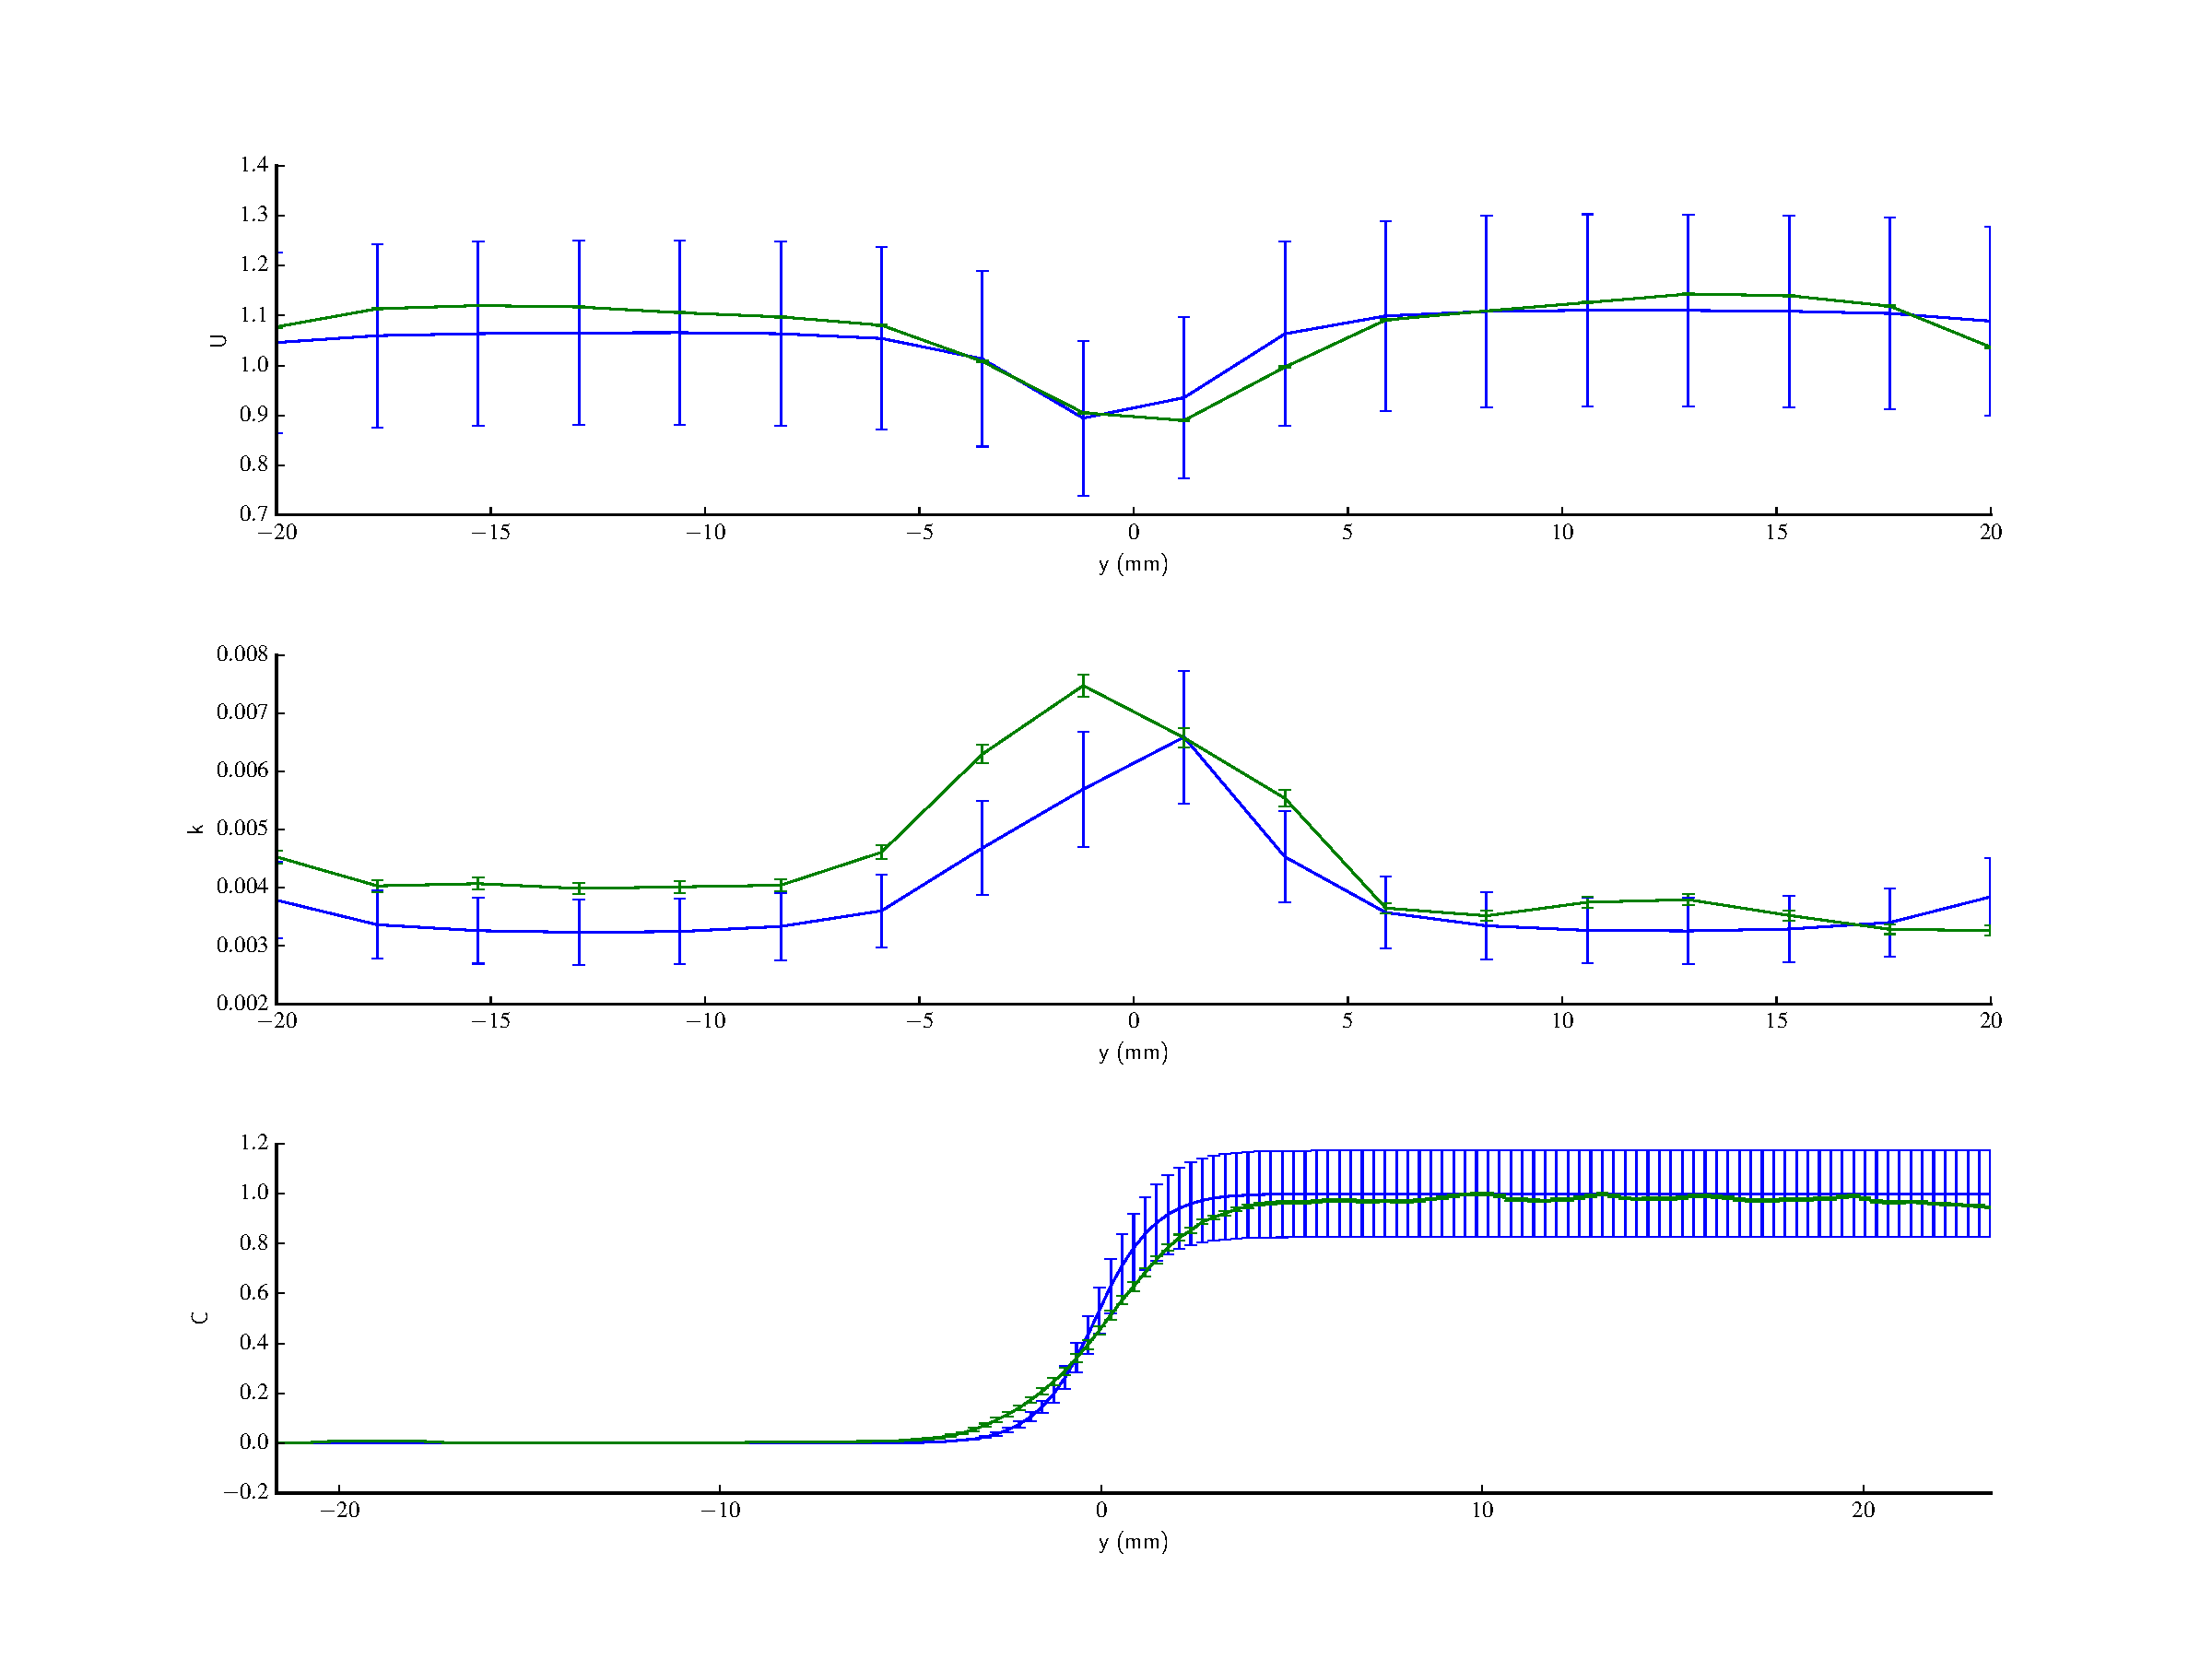
\includegraphics[width=\textwidth]{three_050.pdf}
			\caption{The velocity, turbulent kinetic energy and concentration profiles at \SI{50}{mm} downstream. }
		\end{figure}
		\begin{figure}[h]
			\centering
			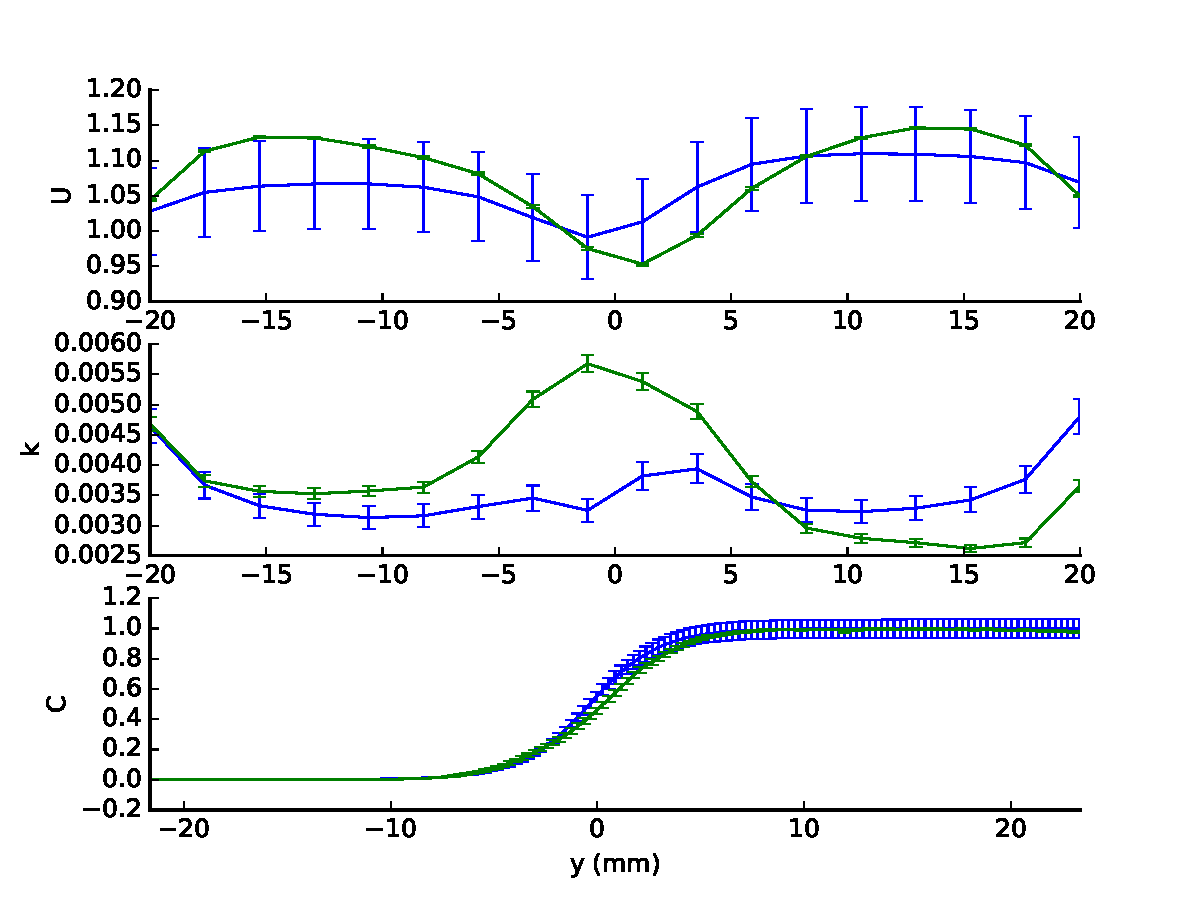
\includegraphics[width=\textwidth]{three_150.pdf}
			\caption{The velocity, turbulent kinetic energy and concentration profiles at \SI{150}{mm} downstream. }
		\end{figure}
		\begin{figure}[h]
			\centering
			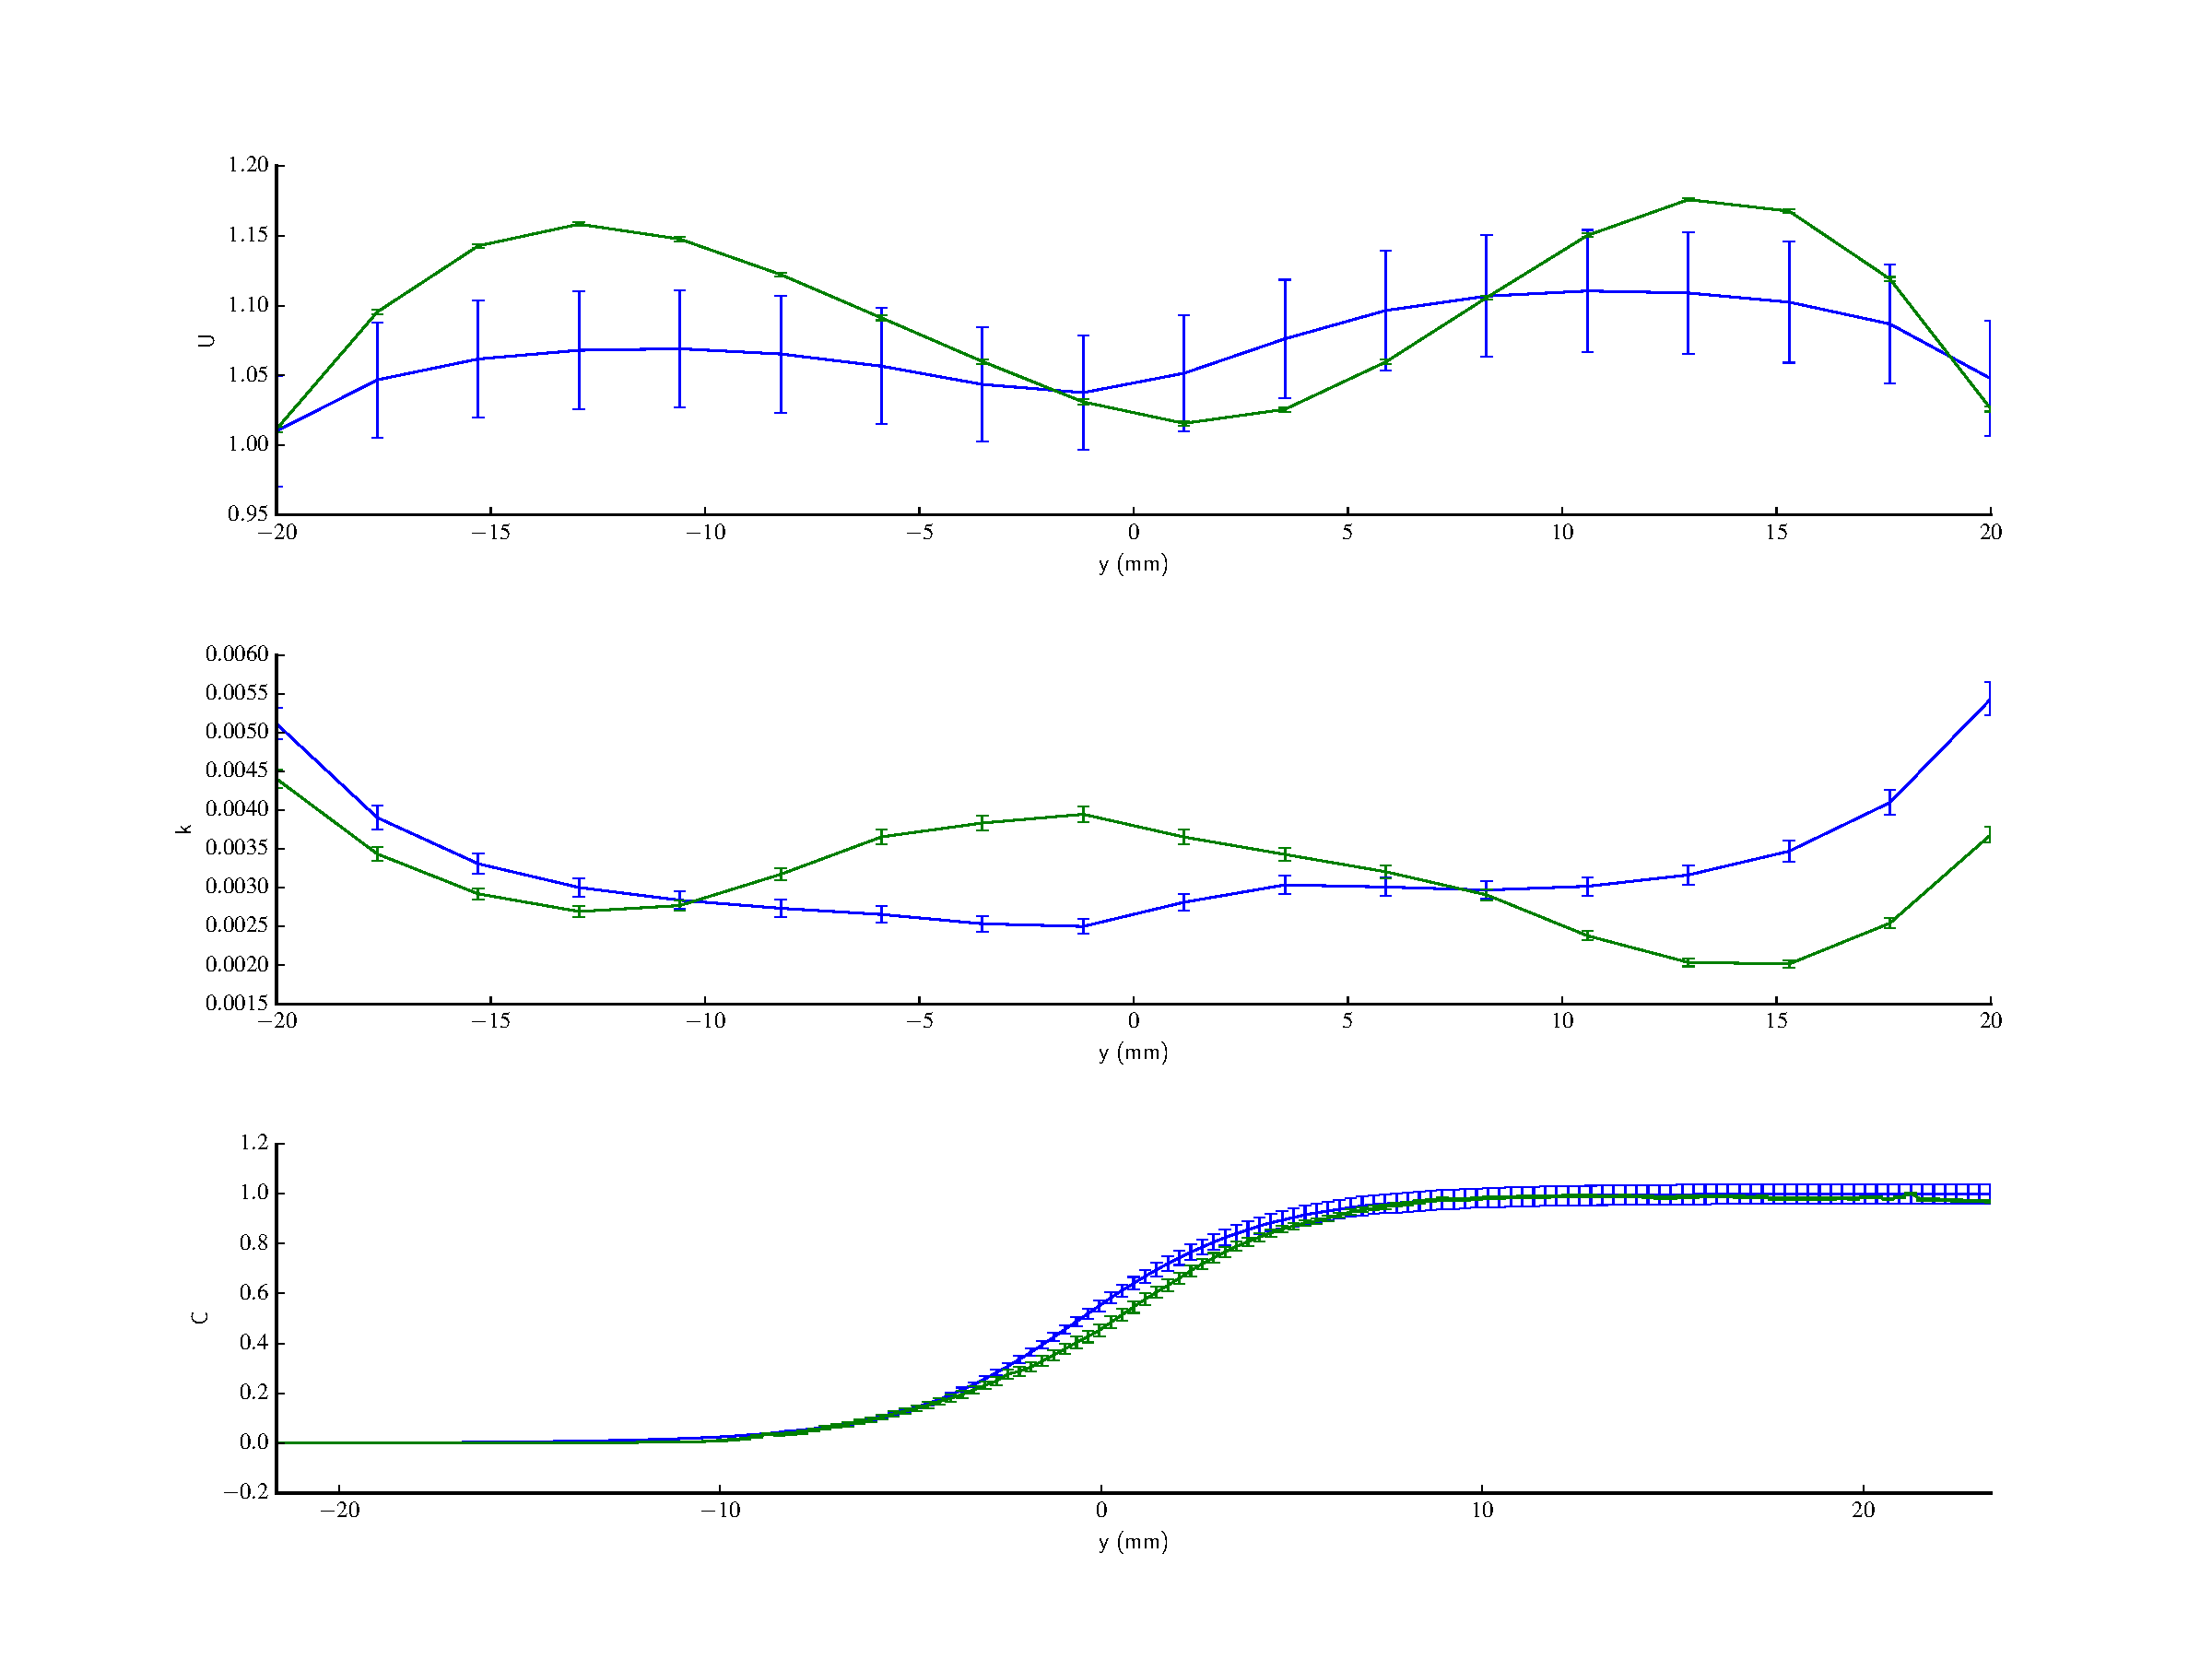
\includegraphics[width=\textwidth]{three_250.pdf}
			\caption{The velocity, turbulent kinetic energy and concentration profiles at \SI{250}{mm} downstream. }
		\end{figure}
		\begin{figure}[h]
			\centering
			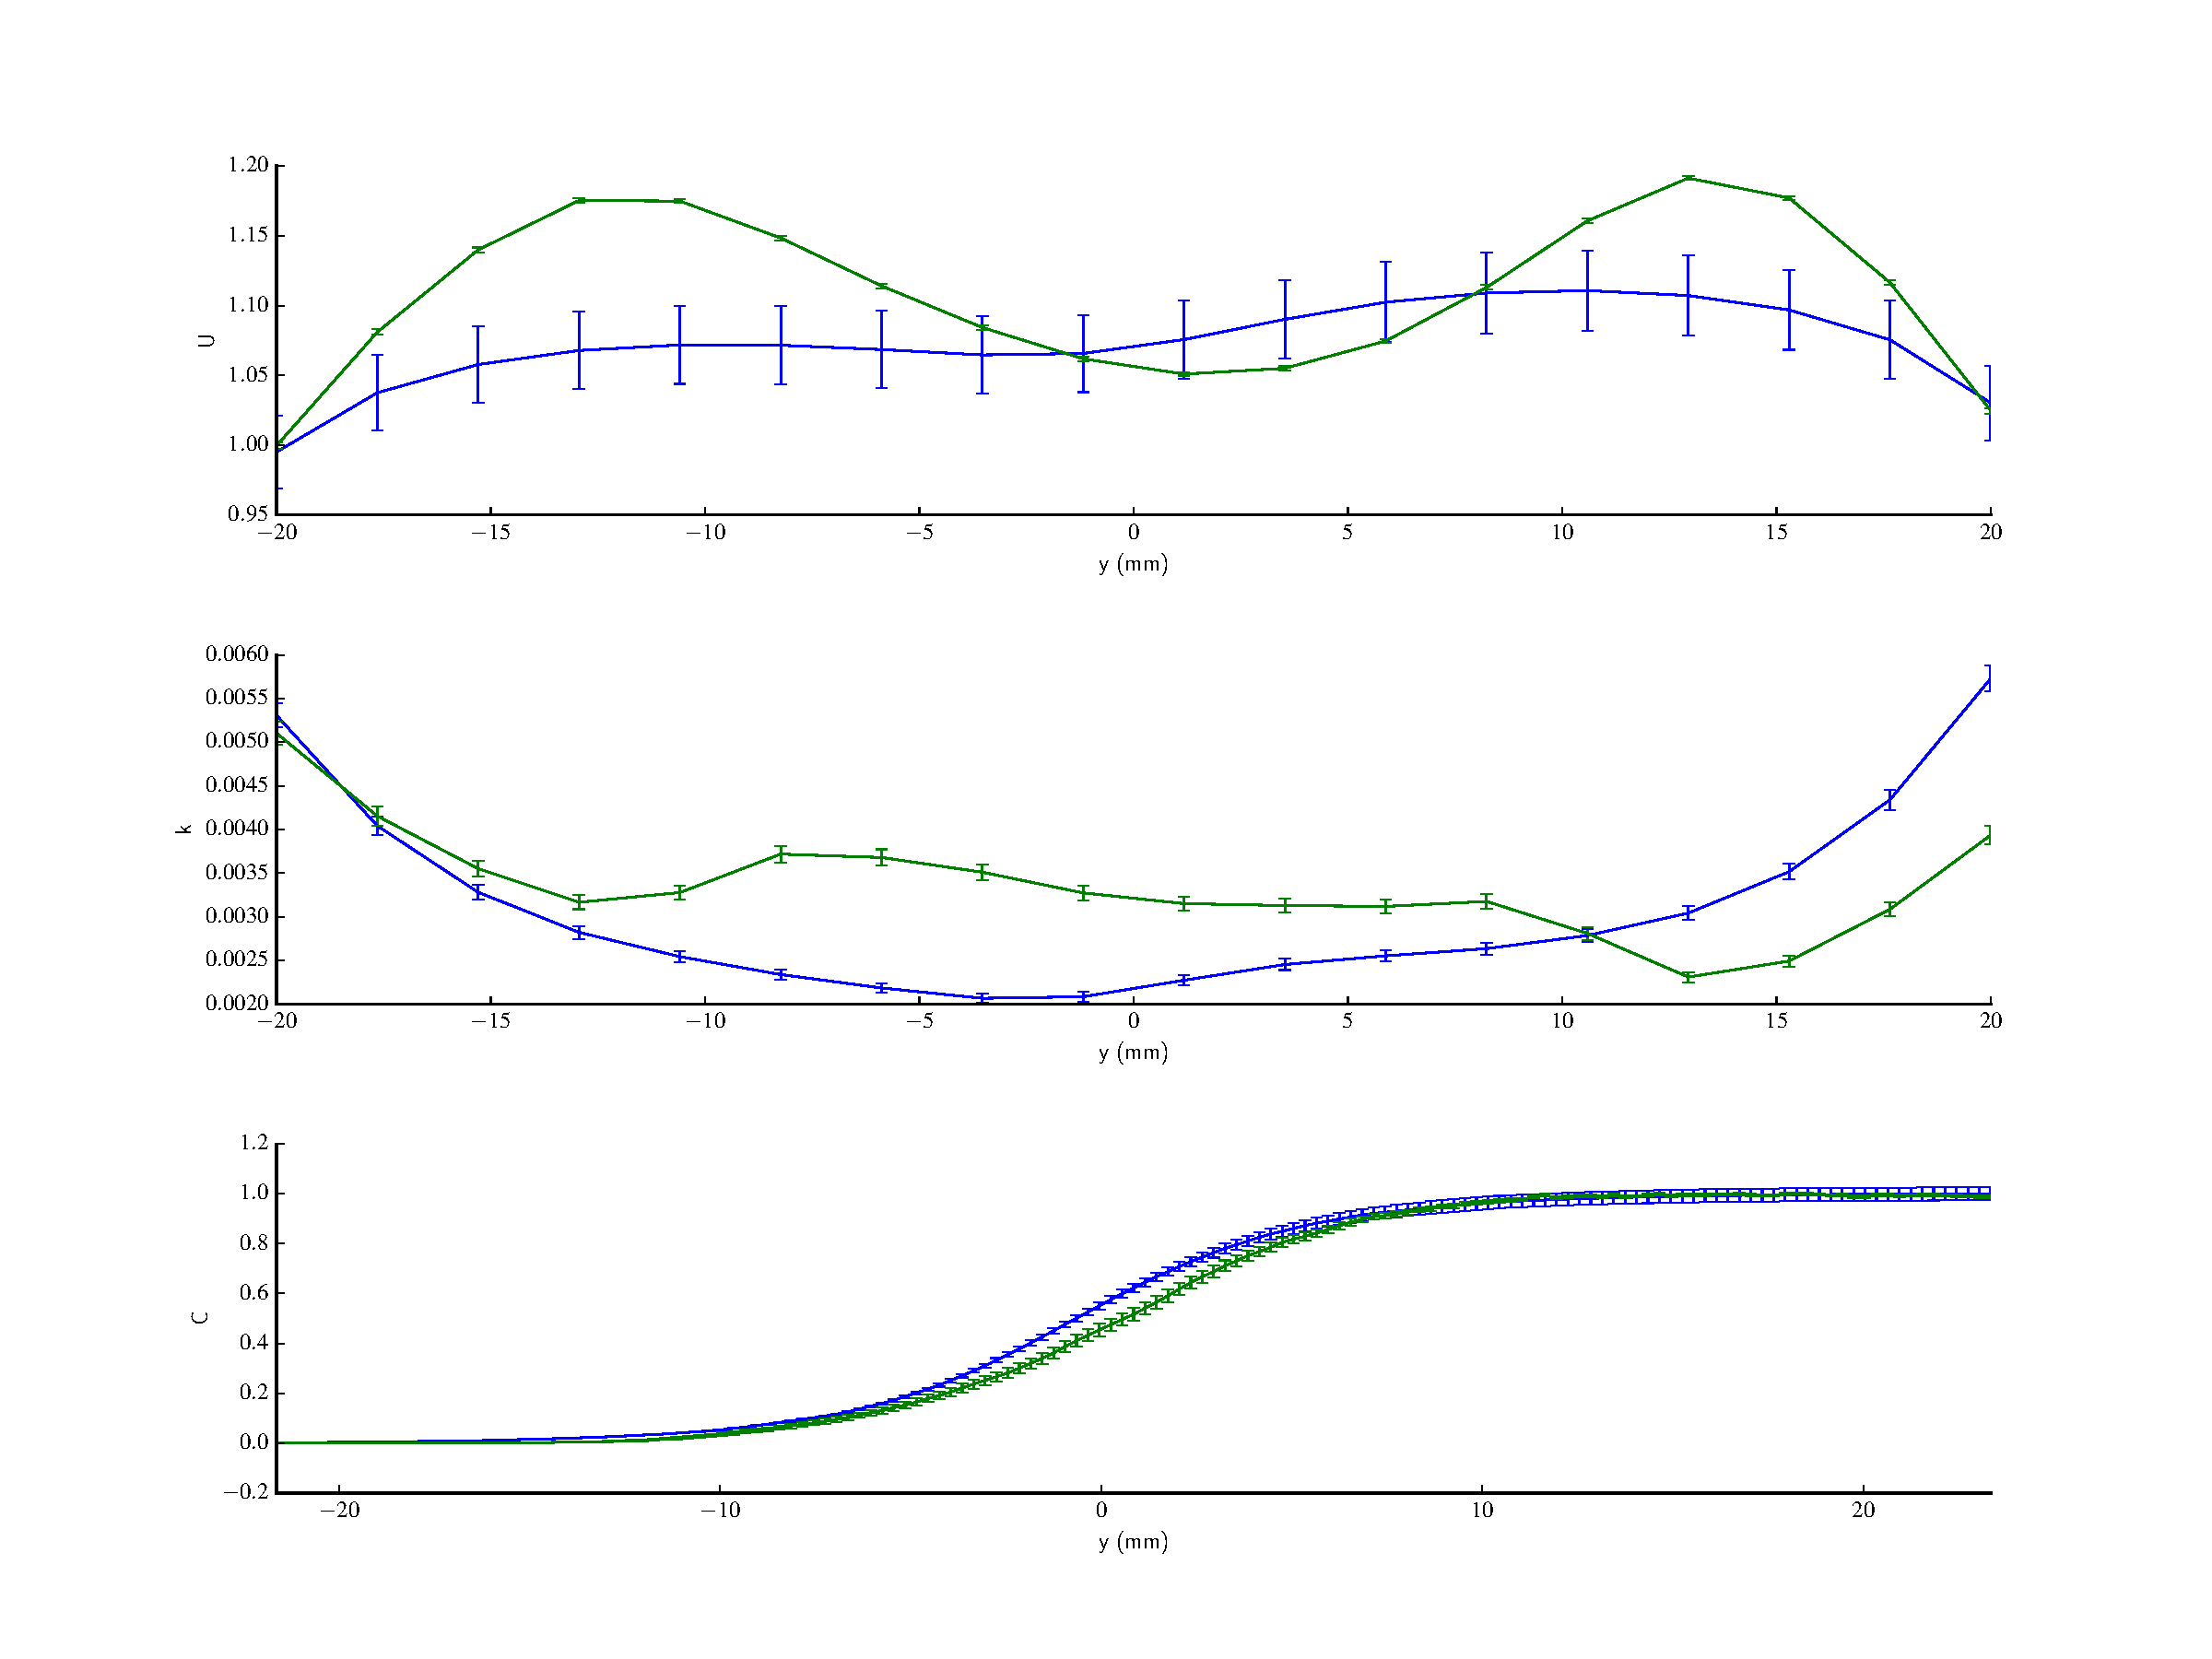
\includegraphics[width=\textwidth]{three_350.pdf}
			\caption{The velocity, turbulent kinetic energy and concentration profiles at \SI{350}{mm} downstream. }
		\end{figure}
		\begin{figure}[h]
			\centering
			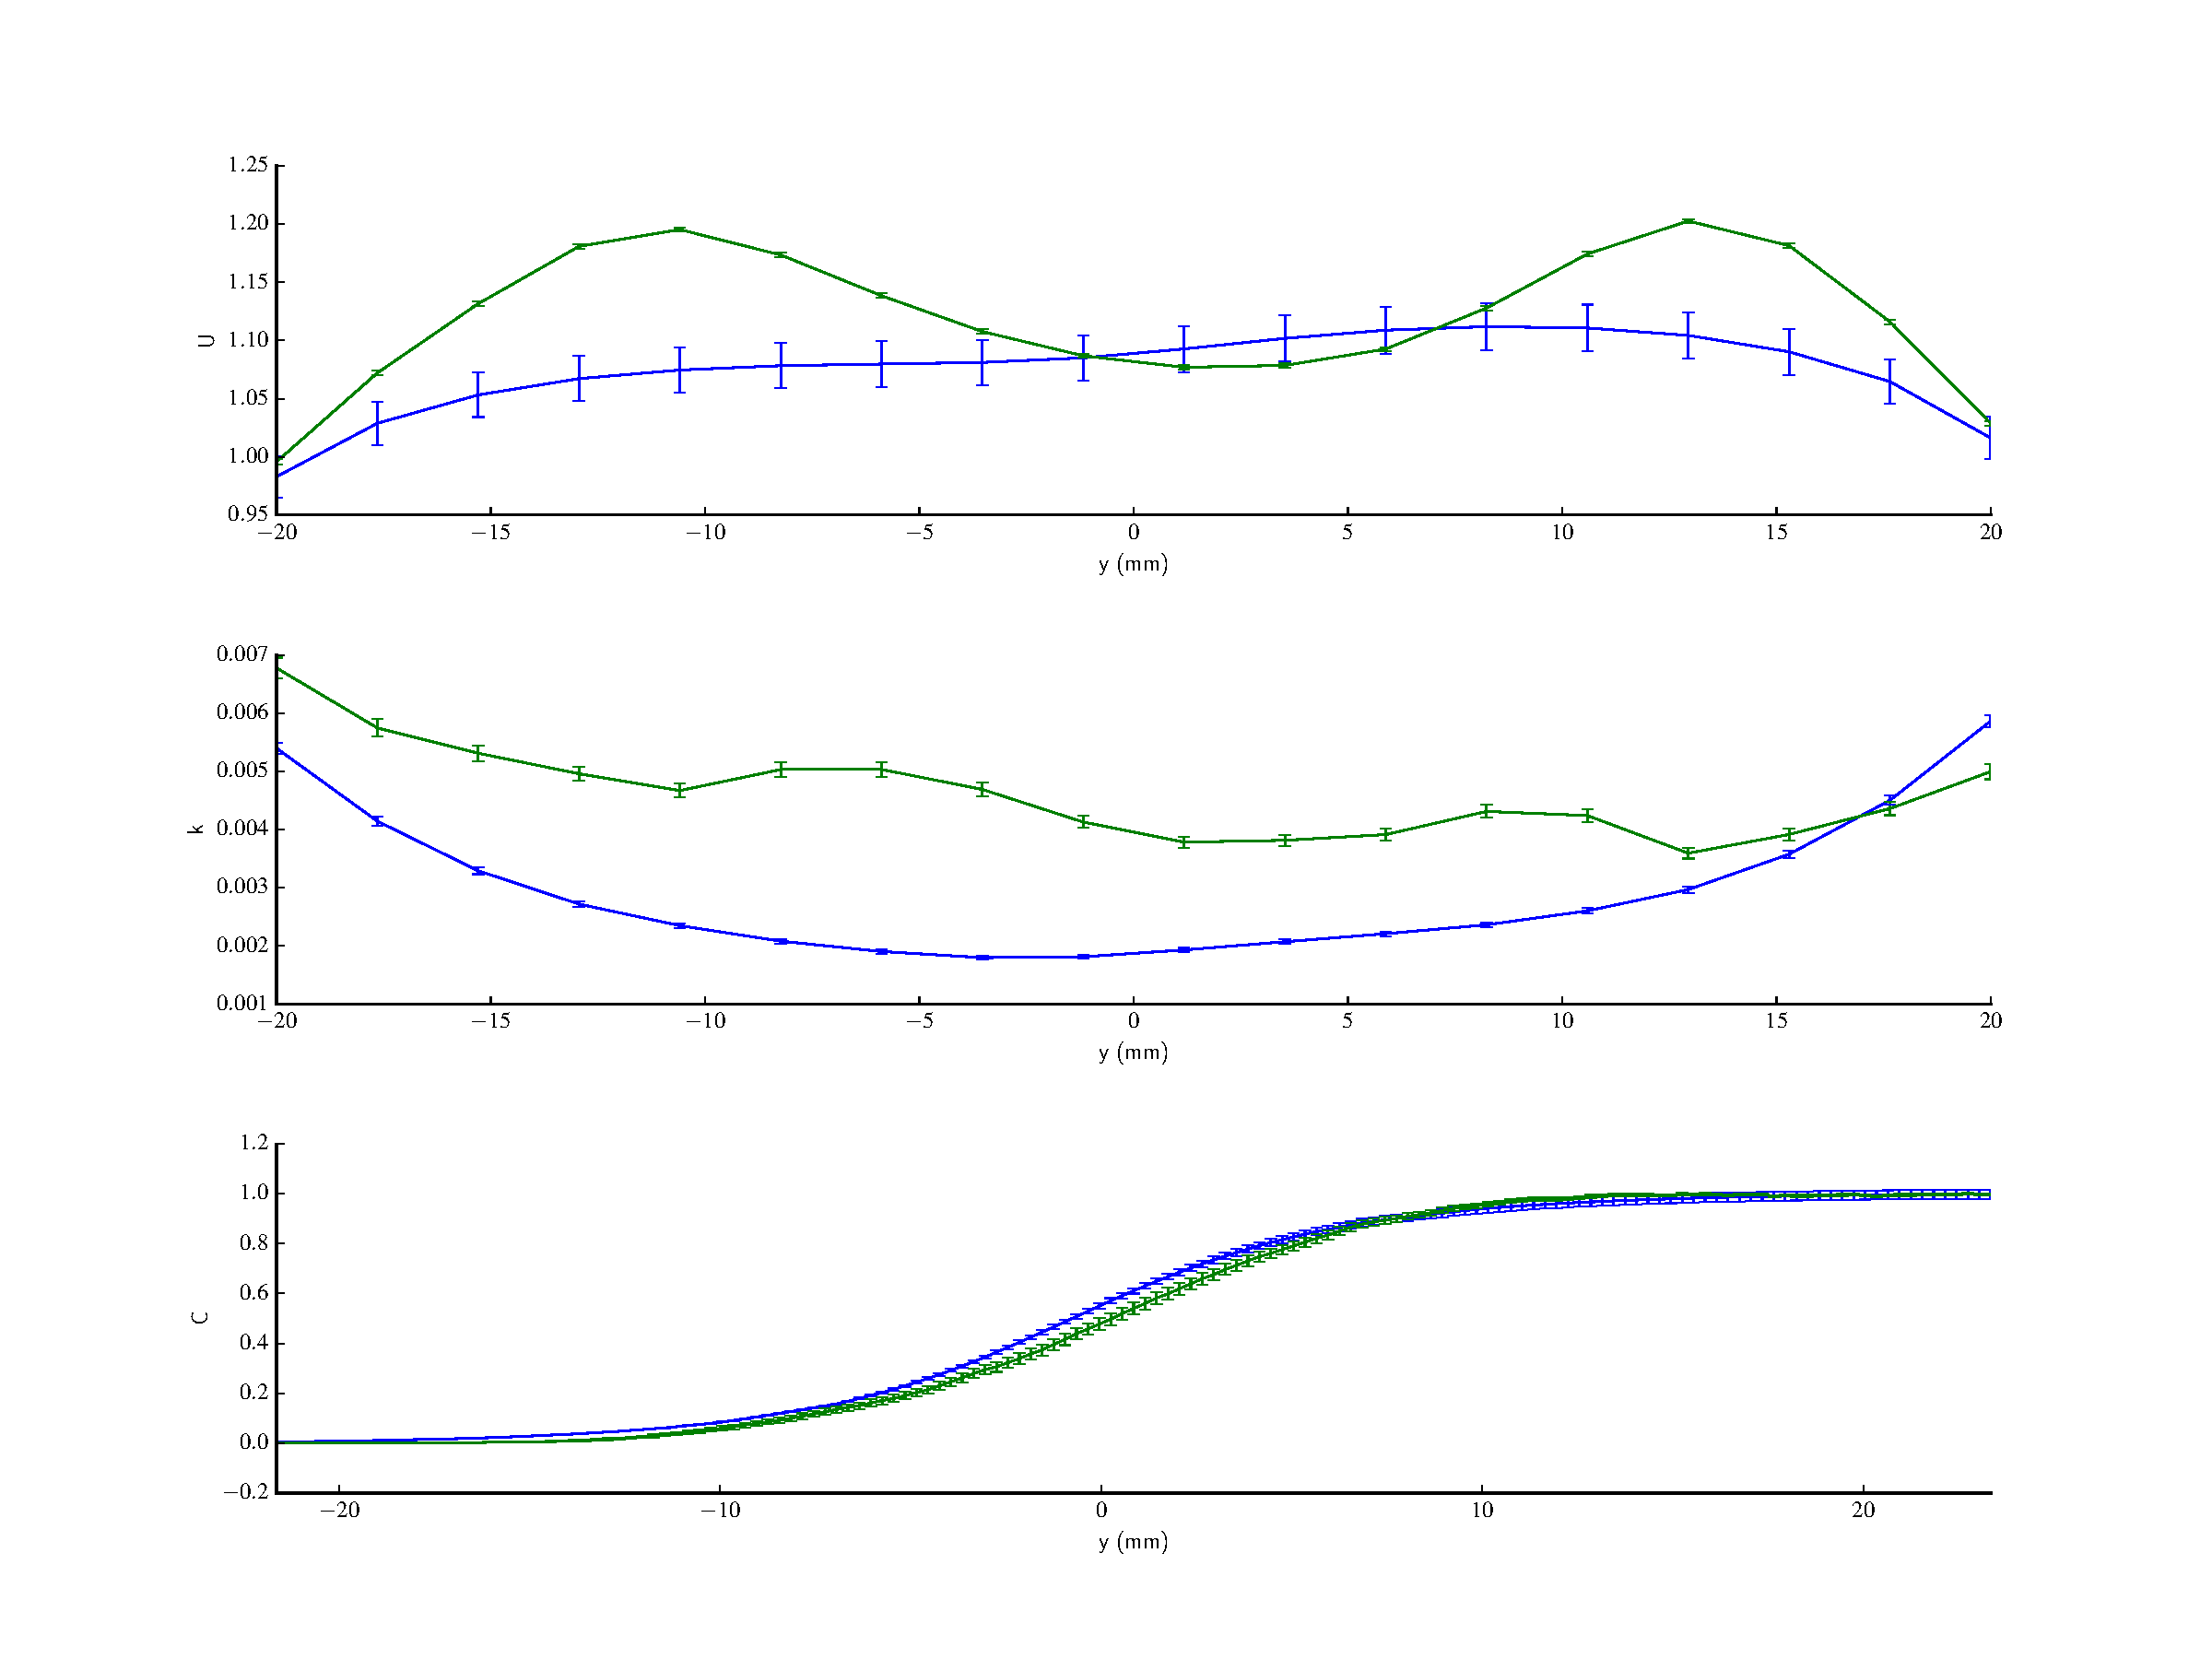
\includegraphics[width=\textwidth]{three_450.pdf}
			\caption{The velocity, turbulent kinetic energy and concentration profiles at \SI{450}{mm} downstream. }
		\end{figure}

\end{appendices}

	\bibliographystyle{unsrtnat}
    \clearpage
	\bibliography{references}

\end{document} % --------------------------------------------------